\section{Problem I}
\textbf{solution}:\\
Let $G'$ be the DAG on the strongly connected components of $G$. Number the nodes of $G^{'}$ in some topological order. We claim that $G$ is semiconnected iff there is always a path from the $i$-th node to the $j$-th node of $G'$ if $i < j$.  

\begin{figure}[h]
	\centering
	\subfloat[Subfigure 1 list of figures text][$G$ is semiconnected]{
		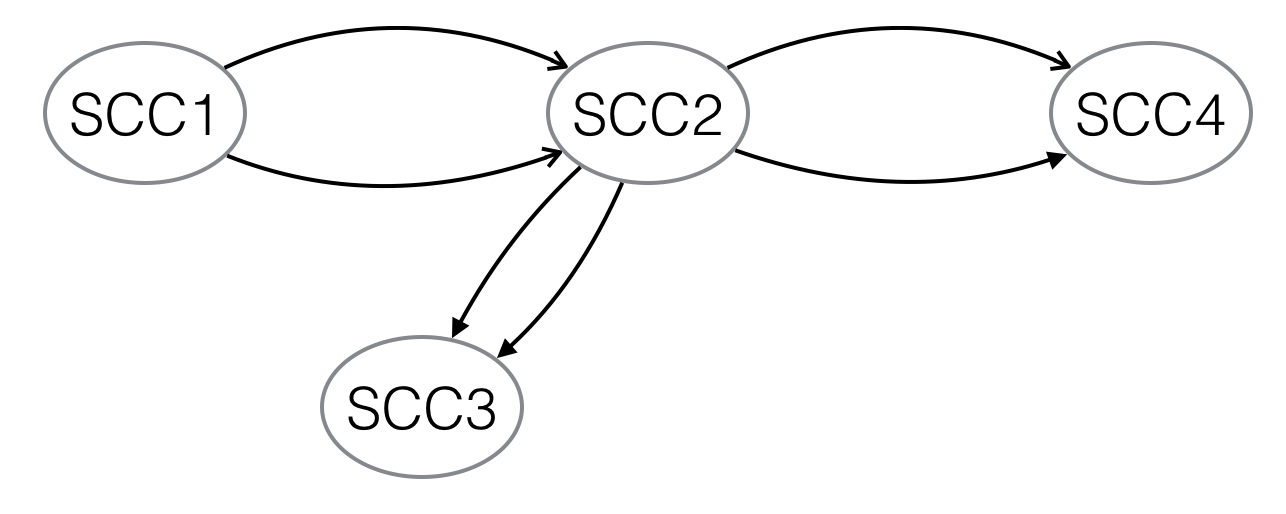
\includegraphics[width=0.4\textwidth]{hw4p1b}
		\label{fg:p1a}}
	\subfloat[Subfigure 2 list of figures text][$G$ is not semiconnected]{
		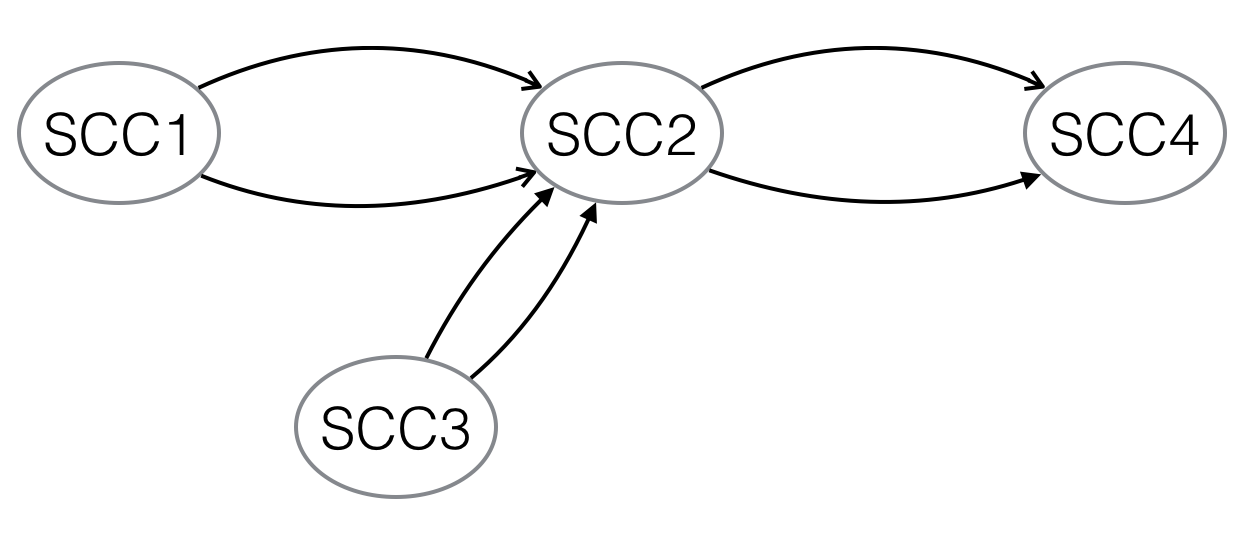
\includegraphics[width=0.4\textwidth]{hw4p1a}
		\label{fg:p1b}}
	\caption{Examples}
	\label{fg:p1}
\end{figure}

Suppose that there is always a path from the $i$-th node to the $j$-th node of $G'$ if $i < j$. Then, for any two vertices $u$ and $v$ in $G$, they either belong to the same SCC (in which case there is a path from $u$ to $v$ and a path from $v$ to $u$), or they belong to two different SCC's, $c_u$ and $c_v$. Without loss of generality, suppose $c_u$ occurs earlier than $c_v$ with respect to the topological order. Then, by hypothesis, there is a path from $c_u$ to $c_v$, so there is a path from $u$ to $v$ as desired. As shown in the Figure \ref{fg:p1a}.\\

Now suppose that for some topological sort of $G'$, there is no path from the $i$-th node (with respect to this sort) to the $j$-th node, where $i < j$. Then, there can be no path from the $j$-th node to the $i$-th node since $i < j$ and the nodes are topologically sorted. Hence, if $u$ is a vertex lying in the $i$-th SCC and $v$ a vertex lying in the $j$-th SCC, there are no paths from $u$ to $v$ or from $v$ to $u$, so $G$ is not semiconnected. As shown in the Figure \ref{fg:p1b}.\\

This observation allows us to devise an algorithm to determine if $G$ is semiconnected: we first compute the strongly connected components of $G$ and construct the graph $G'$ in time $O(\mid V \mid + \mid E \mid)$. Then, using DFS from any vertex in $G'$, we can topologically sort $G'$ in $O(\mid V \mid  + \mid E \mid)$ time. Now, we check if there is a path from the $i$-th SCC to the $j$-th SCC if $i < j$. Note that this is the case iff there is an edge in $G'$ from the $i$-th SCC to the $(i + 1)$-th SCC. Hence, we can just scan through the topological sort in $O(\mid V \mid)$ time to see if the $i$-th SCC has an edge to the $(i + 1)$-th SCC. The total running time of the algorithm is $O(\mid V \mid + \mid E \mid)$.